
\documentclass[UTF8,a4paper,12pt]{ctexart}

\usepackage{geometry}
\usepackage{setspace}
\usepackage{enumitem}
\usepackage{booktabs}
\usepackage{longtable}
\usepackage{array}
\usepackage{amsmath}
\usepackage{graphicx}
\usepackage{tabularx}

\usepackage{xcolor}
\usepackage{hyperref}
\usepackage{titlesec,tikz}
\usetikzlibrary{arrows.meta,positioning,shapes.geometric}


\geometry{left=2.6cm,right=2.6cm,top=2.6cm,bottom=2.6cm}
\setstretch{1.35}
\hypersetup{
    colorlinks=true,
    linkcolor=blue,
    urlcolor=blue,
    citecolor=blue
}
\setlist[itemize]{leftmargin=2em}
\setlist[enumerate]{leftmargin=2em}

\titleformat{\section}{\Large\bfseries}{\thesection}{1em}{}
\titleformat{\subsection}{\large\bfseries}{\thesubsection}{1em}{}

\title{\textbf{inFDT 商业计划书}\\[0.5em]
\large 基于信息传播双边拍卖机制的智能交易撮合平台}
\author{}
\date{}

\begin{document}

\maketitle

\newpage
\tableofcontents

\section{项目概述}


\subsection{项目简介}


inFDT 是一个基于信息传播双边拍卖机制的智能交易撮合平台。

平台以博弈论和机制设计为理论基础，结合 McAfee 双边拍卖、信息传播激励、信用指数、Sybil 风控和标签化分类方法，为买卖双方提供高效、可信、可解释的交易撮合服务。

其只是一个普通的信息展示平台，而是希望通过机制设计解决交易中的真实报价、用户参与、邀请传播、市场定价和风险控制问题。

平台主要面向具有稀缺性、排他性和一次性占用特征的数字资源与金融资源，例如 AI 算力时间片、Agent 任务执行名额、限时 API 优先调用权、专家审核时间片、应收账款与票据收益权等。

并通过双边拍卖完成价格发现与交易撮合，通过信用风控降低虚假账号和恶意操控风险，通过标签化分类解决非完全同质资源难以直接比较的问题。

\subsection{项目定位}

inFDT 的定位可以概括为：

inFDT 定位为一个面向稀缺数字资源与金融资源交易的机制型平台。其核心服务对象不仅普通大众消费品市场，更是供需双方数量有限、资源具有明确占用边界、价格需要动态发现、交易双方存在信任成本的双边市场。

从应用方向看，inFDT 优先服务于 AI 算力、数字服务、专业审核资源、企业金融资产等具有一定标准化基础、但又难以完全统一定价的交易场景。这类资源通常存在供给有限、需求波动明显、人工议价效率低、交易风险较高等问题，适合通过机制化撮合方式提高交易效率。

从平台角色看，inFDT 不直接作为买方或卖方参与交易，而是作为交易机制提供者、价格发现工具和风险筛选基础设施，为买卖双方提供统一、透明、可解释的交易规则。平台的核心价值不在于简单连接供需信息，而在于通过机制设计降低策略操控空间，提高交易匹配效率，并为市场形成可参考的成交价格。

\subsection{核心价值}

inFDT 的核心价值包括四个方面。

\begin{enumerate}
    \item \textbf{提高买卖双方撮合效率。} inFDT 通过双边拍卖机制同时处理买方需求和卖方供给，避免传统平台中单向报价、人工议价或简单信息展示带来的低效问题。平台能够根据买卖双方报价自动确定可成交对象，从而提高交易匹配效率。
    \item \textbf{引导用户真实报价。} 平台以博弈论和机制设计为理论基础，关注激励相容性（IC）。在机制规则下，用户真实表达自身估值或成本是其占优策略，从而减少虚假报价、策略性报价和价格操控行为。
    \item \textbf{保障用户参与意愿。} 平台在机制设计中考虑个体理性（IR），即用户参与交易后的收益不低于不参与交易时的收益。对于买家而言，成交价格不应高于其真实估值；对于卖家而言，成交价格不应低于其最低可接受价格。由此可以增强用户持续参与平台交易的意愿。
    \item \textbf{扩大市场规模并提升交易效率。} inFDT 面向信息传播场景，关注用户之间的邀请关系和传播路径。通过合理的传播激励设计，平台能够鼓励用户邀请更多真实买家和卖家进入交易池，在扩大市场参与规模的同时，提高成交数量和社会福利水平。 \item
    \item\textbf{形成可持续的平台收入。} 平台可以通过 McAfee 类双边拍卖机制形成机制预算盈余，即买方支付价格与卖方获得价格之间的差额。该盈余由公开透明的机制规则产生，可用于平台运营、信用审核、分类评估、风险准备和后续系统建设。
    \item \textbf{提供市场价格发现与定价参考。} inFDT 的机制运行结果不仅可以用于完成交易撮合，还可以沉淀为同类资源的市场价格数据。通过多轮交易结果的积累，平台能够为 AI 算力、数字服务、金融资源等场景提供动态价格参考，降低市场定价不透明带来的交易摩擦。 \end{enumerate}


\newpage
\section{市场痛点与项目机会}

\subsection{传统撮合平台缺少机制设计}

现有许多交易平台主要依赖信息展示、人工撮合、固定价格或简单竞价。这类平台能够帮助买卖双方发现彼此，但往往没有系统处理用户的策略行为。

在双边交易中，买家可能倾向于压低报价，卖家可能倾向于抬高报价。如果平台只依赖人工判断或简单议价，就很难鼓励用户真实表达自身估值，同时也会消耗大量的成本。

inFDT 的项目机会在于：将机制设计引入交易平台，使交易规则本身能够约束和引导用户行为，而不是完全依赖平台人工审核。

\subsection{信息传播场景下市场厚度不足}

很多交易机会并不天然集中在一个公开市场中。尤其在企业服务、供应链金融、算力资源、专家服务和 Agent 任务市场中，真实买方和卖方往往分散在不同组织、行业关系和社交网络中。

如果没有足够的参与者，交易池就会过薄，买卖双方难以匹配，价格也难以真实反映市场供需。

同时，用户可能不愿意主动邀请更多参与者，因为邀请他人可能增加竞争。比如买家邀请更多买家，可能让自己面对更高竞争；卖家邀请更多卖家，可能让自己面对更低成交概率。

因此，平台需要解决一个关键问题：如何让用户在不损害自身合理利益的情况下，愿意扩散交易信息，邀请更多真实参与者进入市场。

\subsection{双边交易中的真实报价问题}

inFDT 面向的是双边市场。买方有最高愿付价格，卖方有最低可接受价格。交易能否发生，取决于买方估值是否足以覆盖卖方成本。

如果用户可以通过虚假报价获得更高收益，平台就会出现报价失真、成交效率下降和价格参考失效等问题。

因此，inFDT 的核心机制需要围绕真实报价、个体理性、交易效率和平台预算平衡展开。具体机制设计由团队在第三章补充，本计划书其他章节只说明平台的商业价值、应用场景和落地方式。

\subsection{稀缺数字资源与金融资源缺少动态定价方式}

AI 和金融科技场景中存在大量具有稀缺性和时间窗口的资源。例如算力高峰期的 GPU 时间片、特定时段的 API 优先调用权、有限的 Agent 任务执行名额、高质量专家审核时间、特定应收账款或票据收益权等。

这些资源具有共同特点：不能无限复制，不能同时完整分配给多个买方，且价值会受到时间、质量、风险和供需关系影响。

传统固定价格、订阅价格或人工议价方式难以处理这些动态变化。inFDT 可以通过双边交易机制，使价格由买卖双方在同类交易池中形成，从而提升资源配置效率。


\newpage
\section{核心机制与产品方案}

本章说明 inFDT 的核心交易机制和产品落地方式。正文部分不展开完整数学证明，而是按照平台实际运行顺序说明：买卖双方如何报价，平台如何定价与匹配，邀请如何产生奖励，balance 扩容如何改善局部供需失衡，以及这些机制如何转化为交易撮合、风控信用和数据服务能力。更形式化的机制定义、符号说明和仿真实验结果见附录 A 与附录 B。

\subsection{机制运行主线：从报价到增量撮合}

inFDT 的核心机制可以概括为一条连续交易链条：买卖双方先进入同质交易池，平台根据预先确定的价格规则筛选可交易主体，再通过随机匹配形成补充前交易；随后平台根据补充前交易分配邀请奖励，并在当前交易池买卖双方失衡时启动 balance 扩容，完成剩余主体的增量撮合。

具体来说，平台首先按照品类、规格、质量等级、交付区域、交付时间和履约要求，将相近的采购需求与供货能力放入同一交易池。买方提交最高可接受价格，卖方提交最低可接受价格。平台并不让双方自由议价，而是先确定本轮买方支付价和卖方收取价，再判断哪些买方和卖方愿意在该价格下交易。满足价格门槛的主体进入候选集合，随后通过随机匹配形成补充前交易。

补充前交易形成后，平台立即锁定这些交易。锁定意味着，后续即使系统为了改善供需结构而补充新的交易主体，也不能替换已经确定的买方或卖方。补充前交易产生的机制盈余，是邀请奖励的主要来源。平台将奖励与真实交易绑定，而不是与注册数量或单纯邀请人数绑定，从而鼓励用户邀请真正有交易需求和履约能力的上下游主体。

完成补充前交易和奖励确认后，平台再检查当前交易池是否存在买卖双方失衡。如果某一侧明显不足，系统只从下一层邀请网络中补充当前缺失方。例如，卖方不足时，只从当前买方直接邀请的下一层卖方中补充；买方不足时，只从当前卖方直接邀请的下一层买方中补充。补充完成后，平台只对原始池中尚未匹配的主体和补充主体继续进行增量撮合。由此，inFDT 将“邀请奖励”和“效率扩容”分开：前者奖励真实扩散贡献，后者提升当前层流动性和平台可持续收入。

整体流程如图~\ref{fig:infdt-mechanism-flow} 所示。

% 这里保留你现有的 tikz 流程图
% \begin{figure} ... \end{figure}

图~\ref{fig:infdt-mechanism-flow} 展示了每一轮机制的执行顺序。左侧部分对应补充前交易形成过程：平台先定价，再筛选可交易主体，再通过随机匹配形成补充前交易，并将其盈余用于邀请奖励。右侧部分对应 balance 扩展过程：只有当原始交易池不满足 balance 阈值时，平台才从下一层补充缺失方，并对剩余主体进行增量匹配。这样，邀请奖励与补充前真实交易绑定，而 balance 补充主要承担提高流动性和增加平台收益的功能。

\subsection{关键机制设计}

\subsubsection{滞后定价与随机匹配}

inFDT 的第一项关键设计是将“价格形成”和“当前报价”适度分离。若当前轮价格直接由当前轮报价决定，买方可能故意压低报价，卖方可能故意抬高要价，从而使报价变成策略性试探工具。为减少这种操纵空间，平台采用滞后定价思想：当前轮价格不直接依赖当前轮报价，而是由更早的历史信息、基准价格或预设规则确定。

在价格确定后，报价只用于判断交易资格。买方报价达到买方支付价，说明其愿意在该价格下采购；卖方要价不高于卖方收取价，说明其愿意在该价格下供货。理论模型中，所有满足价格门槛的主体采用等概率随机匹配，因此用户不能通过报得更高或更低来获得更高排序。在真实系统中，平台可以在不改变主机制逻辑的前提下，引入信用加权匹配：履约记录更好、风险更低、平台可信度更高的主体获得更高匹配概率。

这一设计的作用是让报价回归交易意愿表达，而不是排序竞争工具。用户想提高长期成交机会，应依靠稳定履约、真实交易和低风险行为，而不是依靠策略性报价。

\subsubsection{交易锁定与邀请奖励}

inFDT 的第二项关键设计是先锁定补充前交易，再发放邀请奖励。在每轮交易中，平台先在原始交易池中形成补充前交易集合。该集合一旦确定，就不再被后续补充主体替代。这样可以保护已经形成的交易结果，也避免用户担心后续新主体进入后推翻原成交。

邀请奖励只来自补充前已经能够形成并最终履约完成的交易。平台将单笔交易的可分配盈余拆分为买方侧奖励池和卖方侧奖励池，分别奖励该笔交易中买方和卖方的有效直接邀请者。如果同一侧存在多个有效邀请者，则在该侧内部平分；如果没有有效邀请者，则对应奖励池可由平台保留或进入公共奖励池。

这一设计避免了“注册即奖励”的粗放拉新模式。邀请者获得收益的前提不是带来一个账号，而是带来能够真实参与交易并完成履约的主体。这样，邀请机制服务于真实市场扩展，而不是流量补贴。

\subsubsection{Balance 扩容与新增收益}

inFDT 的第三项关键设计是动态供需平衡扩容。分层邀请网络中，某一轮交易池可能出现买方多而卖方少，或者卖方多而买方少的局部失衡。若平台只在原始池中被动撮合，许多潜在交易会因为缺少对手方而无法发生。

因此，平台在补充前交易锁定后，再判断当前交易池是否失衡。当某一侧明显不足时，系统识别缺失方，并只从下一层中补充由当前层相反类型主体直接邀请的缺失方主体。该规则有两个限制：第一，不跨多层任意搜索；第二，不按照报价高低选择补充对象。这样可以避免 balance 扩容成为新的报价操纵渠道。

补充完成后，平台只让原始池中尚未匹配的主体与补充主体进行增量撮合。与补充前交易不同，balance 补充后新增交易的盈余不进入本轮邀请奖励池，而由平台保留，用于覆盖撮合、风控、履约保障和系统运营成本。也就是说，补充前交易承担“邀请激励”功能，补充后新增交易承担“效率提升与平台收益”功能。

\subsection{产品落地方案}

围绕上述机制，inFDT 的产品方案分为三层：交易撮合层、风控信用层和数据服务层。交易撮合层面向买方和卖方，完成需求发布、报价提交、交易池划分、定价、匹配、交易锁定和增量撮合；风控信用层负责邀请关系记录、履约评价、防女巫检测和风险分层；数据服务层则将真实交易过程沉淀为价格指数、信用画像、交易网络风险报告和供应链金融数据接口。

\begin{table}[htbp]
    \centering
    \renewcommand{\arraystretch}{1.25}
    \begin{tabular}{p{0.22\linewidth}p{0.68\linewidth}}
        \hline
        \textbf{产品层次} & \textbf{主要功能}                                                                                                \\
        \hline
        交易撮合层         & 买方发布采购需求、提交最高可接受价格、查看历史价格并完成验收评价；卖方发布供货能力、提交最低可接受价格、管理订单并积累履约信用；平台撮合引擎负责交易池划分、定价、筛选、随机匹配、交易锁定和 balance 增量撮合。 \\
        风控信用层         & 记录邀请关系和交易履约情况，识别小号注册、循环邀请、互评刷分、异常邀请树和低外连高内聚社群，并对高风险主体采取奖励递延、评价降权、提高保证金、交易限额和人工审核等措施。                         \\
        数据服务层         & 基于订单、报价、成交价、履约、支付、评价和邀请关系数据，形成区域采购价格指数、品类价格趋势、企业信用画像、交易网络风险报告和供应链金融数据接口。                                     \\
        \hline
    \end{tabular}
    \caption{inFDT 产品方案分层}
\end{table}

在产品落地中，买方端降低采购询价和比价成本，卖方端降低获客成本并通过履约信用获得更多交易机会，平台端则通过撮合、风控和数据服务形成长期价值。inFDT 本身不直接放贷，而是向银行、保理公司、小贷公司等持牌机构提供可信交易数据和风控报告，支持订单融资、应收账款融资、采购贷和小微企业信用贷等服务。

\subsection{效率验证摘要}

为验证机制有效性，我们将未启用 balance 的基础机制作为 baseline，将启用动态供需平衡扩容的机制作为优化方案进行仿真比较。实验采用随机供应链社交森林，模拟不同市场规模下买方、卖方和邀请关系的形成过程，并比较成交数量、增量社会福利效率、总社会福利效率、balance 改善幅度和补充成本。

现有仿真结果显示，启用 balance 后，机制在不同市场规模下均提高了增量福利效率和平均成交数量。例如，在 \(N=1000\) 的市场规模下，baseline 的平均增量福利效率约为 0.794，启用 balance 后提升至约 0.889；平均成交数量也从约 158.3 提升至约 184.3。同时，balance 机制降低了增量福利效率方差，说明平台表现不再过度依赖随机网络结构，撮合结果更加稳定。详细实验设置、指标定义和结果表格见附录 B。

\section{平台增强模块}

第三章机制是平台核心，但真实商业落地还需要增强模块支撑。交易平台难免会出现“信用不好的用户”，同时社交网络下的机制也会导致恶意开创小号谋利等女巫风险。
同时，针对物品难以达到双边拍卖的同质要求。因此我们必须要量化可信度和风险，同时引入标签分类化模式以达到“类同质”的效果。

inFDT 的增强模块主要包括资源准入、标签化分类、信用指数、Sybil 风控、评测 Agent 和人工复核机制。

具体的公式理论放在附录里可供查看。



\subsection{标签化分类与类同质交易池}

双边拍卖需要同质化的物品，但现实生活中很多物品难以实现同质化。因此我们设定“类同质”这个概念，
即把具有一定相似性的特质或者质量处于相同区间的物品定义为“类同质”，便向看作等价的同类物品，可以放在同一场双边拍卖交易中。

而标签化分类模块可以用于解决非完全同质资源难以直接拍卖的问题。

平台可以根据资源类型设置不同标签。例如：

\begin{itemize}
    \item AI 算力时间片可以按照 GPU 型号、区域、时间窗口、服务等级、可用时长和稳定性分类。
    \item Agent 任务执行名额可以按照任务类型、Agent 成功率、执行延迟、稳定性、安全性、行业适配度和历史反馈分类。
    \item 应收账款与票据收益权可以按照债务人信用、期限、核心企业确认程度、历史回款记录、材料完整性和风险等级分类。
\end{itemize}

分类后，平台将相似资源放入同一个类同质交易池中，再运行主机制。这样可以避免差异过大的资源直接比较，减少价格失真和交易纠纷。



\subsection{信用指数模块}

信用指数用于衡量用户在平台中的行为可靠性。平台不应只依赖用户互评，因为用户评分容易被互刷、小号和团伙操控影响。

inFDT 的信用指数应重点考虑以下信息：

\begin{enumerate}
    \item 用户评分。来自买卖双方互评，但评价者本身也需要经过可信度加权。
    \item 平台打分。来自平台记录、抽查、仲裁、规则核验和履约事实。
    \item 交易成功比例。反映用户是否真实完成交易，是否经常取消、违约或导致纠纷。
    \item 账号成熟度。用于缓解冷启动问题，防止新账号通过少数交易或少数好评快速获得过高信用。
\end{enumerate}

在商业表达中，可以将信用指数解释为：平台对用户历史行为、履约能力和交易可靠性的综合评价。该指数可以影响用户进入交易池的权限、保证金要求、审核强度、邀请权重和交易优先级。

\subsection{Sybil 风控模块}

Sybil 风控用于判断账号是否可能是小号、虚假账号或被同一主体控制的账号。它与信用指数不同：信用指数回答“这个用户表现好不好”，Sybil 风险回答“这个账号是否可能不真实或被操控”。

inFDT 的 Sybil 风控可以从三个方面识别风险：

\begin{enumerate}
    \item 信息一致性异常。包括身份信息冲突、收款账户重复、地址异常复用、资料频繁变更、证明材料高度相似等。
    \item 设备、地点和时间异常。包括同一设备短时间注册多个账号、同一 IP 下大量账号互相邀请、多账号登录时间高度同步、多账号频繁切换同一组设备等。
    \item 邀请关系图与交易图异常。包括星型小号树、异常长链邀请、同父互评团、低活跃叶子节点、封闭互评社区、内部交易闭环等。
    \item 提交的个人信息是否准确全面。包括身份证认证、人脸识别等其他基本信息的登录。
\end{enumerate}

平台早期社交网络不完整，可以先检测明显的树状异常和行为异常；中期可以检测局部团伙结构；成熟期可以引入可信种子和网络信任传播方法。

\subsection{评测 Agent 与人工复核机制}


评测 Agent 的作用分为两部分。

作用一，很多商品不能单纯的依靠离散的标签进行分类。因为我们引入agent评测功能，以此给商品进行评分，通过设计评分区间来对物品进行分类。
我们通过收纳用户的需求和专业人员给出来的评价体系和标准，写一份专门用于agent评价该类特定物品的使用的skills，来规范和训练agent对于该物品的评价。

作用二，对于信用指数模块的平台打分环节以及sybil分控模块。这些板块很多取决于固定的参数和模型。比如说，卖家交货是否及时，信息是否高度重复以及特定的图形结构检测。
这些单一机械的判断可以交由agent来审核，大大减少人力消耗。


同时为了降低误判风险，平台保留人工复核和用户申诉机制。对于高价值交易、高风险账号和争议交易，不能完全依赖自动评分，应进入人工审核或专家复核流程。



\newpage
\section{应用场景与目标客户}

\subsection{场景选择原则}

inFDT 的早期场景不宜过于分散，应选择最能体现“稀缺资源 + 双边报价 + 信息传播 + 信用风控”的场景。

优先场景应满足以下条件：

\begin{enumerate}
    \item 资源具有明确稀缺性。例如时间片、任务名额、收益权、审核名额等。
    \item 资源具有明确交割边界。买方买到什么、卖方交付什么必须清晰。
    \item 资源可以分类或标准化。至少可以通过标签、评分或分层形成类同质交易池。
    \item 买卖双方都存在真实需求。平台需要同时吸引供给方和需求方，否则交易池无法形成。
    \item 信用和履约可以被验证。早期不宜选择过于难以验证、争议过高或合规成本过大的场景。
\end{enumerate}

基于以上原则，inFDT 可以采用“主场景 + 拓展场景”的结构：先聚焦少数主场景完成验证，再逐步扩展到更多资源类型。

\subsection{第一主场景：AI 算力时间片交易}

\subsubsection*{场景描述}

AI 训练、推理、模型评测、批量生成、金融风控和 Agent 执行任务都需要算力。算力需求具有明显波动性：某些时间段需求集中，而一些机构的 GPU、CPU 或推理资源可能处于闲置状态。

inFDT 可以将算力资源拆分为标准化时间片，在同一型号、同一区域、同一时间窗口、同一服务等级的交易池内完成撮合。

\subsubsection*{交易对象}

交易对象是某一时间窗口内的标准化算力使用权，例如：

\begin{itemize}
    \item 同一型号 GPU 的固定时长使用权；
    \item 同一服务等级的推理容量；
    \item 某一时间段内的边缘计算资源；
    \item 某一批 Agent 推理任务所需的算力额度。
\end{itemize}

\subsubsection*{买方}

买方可以包括 AI 公司、模型训练团队、Agent 平台、金融风控系统、科研团队和数据分析机构。

\subsubsection*{卖方}

卖方可以包括云服务商、企业私有 GPU 集群、实验室闲置算力、数据中心和边缘计算节点。

\subsubsection*{为什么适合 inFDT}

AI 算力时间片具有较强的同质性、稀缺性和时间属性。相同型号、区域、时间段和服务等级下的算力可以被划入同一交易池。一个算力时间片一旦被某个买方占用，就不能同时完整分配给其他买方，因此适合用双边交易机制进行分配和定价。

同时，闲置算力和临时算力需求往往分散在不同机构中，适合通过信息传播机制扩大市场厚度。

\subsubsection*{平台价值}

对买方而言，平台可以帮助其在特定时间窗口内找到合适算力资源，减少临时需求无法满足的问题。

对卖方而言，平台可以帮助其提高闲置资源利用率，将未充分使用的算力时间片转化为收益。

对平台而言，该场景相对容易解释，资源边界较清晰，适合作为早期主场景之一。

\subsection{第二主场景：Agent 任务执行名额交易}

\subsubsection*{场景描述}

高质量 Agent 服务并不是无限可复制的软件。Agent 执行任务会消耗推理算力、工具调用额度、私有知识库访问权、任务队列容量，甚至需要人工复核。因此，某类 Agent 在特定时间段内可承接的任务数量是有限的。

inFDT 可以将 Agent 服务转化为“任务执行名额”，在按能力、任务类型和服务等级划分的交易池中进行撮合。

\subsubsection*{交易对象}

交易对象是某类 Agent 在某一时间段内可承接的任务执行名额，例如：

\begin{itemize}
    \item 金融报告分析 Agent 的深度报告处理名额；
    \item 合同审查 Agent 的合同审核名额；
    \item 代码审查 Agent 的 PR 审查名额；
    \item 供应链风险 Agent 的企业风险分析名额；
    \item 数据清洗 Agent 的数据集处理名额。
\end{itemize}

\subsubsection*{买方}

买方可以包括企业客户、个人开发者、任务分发平台、金融机构、软件开发团队和其他 Agent 系统。

\subsubsection*{卖方}

卖方可以包括 Agent 服务商、专业 Agent 开发者、拥有行业知识库的企业和专家 + Agent 混合服务团队。

\subsubsection*{为什么适合 inFDT}

Agent 任务执行名额具有任务一次性和服务容量稀缺的特点。高质量 Agent 的执行能力、任务队列和复核能力有限，不能无限承接任务。

同时，不同 Agent 的能力差异较大，必须先通过评分分层形成类同质交易池。例如可以按照任务成功率、执行延迟、稳定性、安全性、工具调用准确率、用户反馈和行业适配度进行分类。

\subsubsection*{平台价值}

对买方而言，平台可以帮助其在关键时间获得可靠 Agent 服务。

对卖方而言，平台可以帮助优质 Agent 服务方被更多真实需求发现。

对平台而言，该场景具有前沿性，能够体现 Agent economy 下任务能力、服务名额和智能资源的市场化配置价值。

\subsection{第三主场景：应收账款与票据收益权交易}

\subsubsection*{场景描述}

在供应链金融中，应收账款、票据、订单收益权等金融资产具有明确的权利边界。企业可以将未来回款权转让给资金方，以获得现金流支持。

这类资源不同于可复制数据。一笔应收账款或票据收益权如果已经转让给一个资金方，就不能再重复出售给另一个资金方，否则会形成重复融资或欺诈风险。

\subsubsection*{交易对象}

交易对象可以是一笔应收账款、票据贴现权、订单未来回款权或保理资产转让权。

\subsubsection*{买方}

买方可以包括银行、保理公司、小贷机构、产业基金、资产管理机构和其他资金方。

\subsubsection*{卖方}

卖方可以包括供应商、中小企业、持票企业、订单持有人和供应链服务商。

\subsubsection*{为什么适合 inFDT}

应收账款与票据收益权具有一次性、排他性和金融属性。一笔权利转让后不能重复出售，适合通过权属记录、交易记录和风控审核进行交割控制。

同时，不同金融资产风险差异较大，需要按照债务人信用、期限、核心企业确认程度、历史回款记录和材料完整性进行评分分层，形成不同风险等级的类同质资产池。

供应链上下游天然存在企业关系网络，也适合通过信息传播机制发现更多真实资产方和资金方。

\subsubsection*{平台价值}

对中小企业而言，平台可以帮助其更高效地接触资金方，改善现金流。

对资金方而言，平台可以帮助其发现更多经过分类和审核的资产机会。

对平台而言，该场景与金融科技、供应链金融和普惠金融方向结合紧密，适合作为金融科技主场景。

\subsection{拓展场景}

在主场景验证成熟后，inFDT 可以逐步拓展以下场景。

\begin{enumerate}
    \item 限时 API 优先调用权。适用于金融风控 API、企业知识库检索 API、Agent 工具调用通道、实时行情分析 API 等场景。交易对象是某一时间窗口内的优先调用容量。
    \item 专家审核与人机协同评估时间片。适用于模型安全测试、数据质量评估、金融合规审查、供应链资产尽调、合同审核和 Agent 输出人工复核等场景。交易对象是专家或审核团队在某一时间窗口内的审核名额。
    \item 本地模型更新贡献名额。适用于联邦学习、多智能体训练和行业模型共建。交易对象不是可复制的模型更新文件，而是某一轮训练中被纳入全局模型聚合的一次贡献名额。
    \item 未来数据采集任务。适用于未来某一时间窗口内的真实场景数据采集。平台不交易已有数据副本，而是交易未来采集任务名额。
    \item AI 模型安全红队测试名额。适用于模型上线前安全测试、隐私泄露测试、工具滥用测试和金融合规测试。交易对象是一次完整测试服务或测试名额。
\end{enumerate}


\section{商业模式与成本结构}

\subsection{收入来源}

inFDT 当前阶段的主要收入来源应围绕机制预算盈余和交易服务展开。

\paragraph{第一，机制预算盈余。}
双边交易机制运行后，买方支付价格与卖方获得价格之间可能形成差额。该差额不应表述为平台随意赚差价，而应表述为机制预算盈余、撮合价差留存或交易服务留存。它来源于公开、透明的机制规则，可以用于平台运营、信用审核、分类评分、风险准备和系统维护。

\paragraph{第二，交易服务费。}
平台可以对成功撮合的交易收取服务费用。具体费率不在本计划书中虚构，应根据试点场景、交易金额、履约成本和用户接受度进一步测算。

\paragraph{第三，企业服务费。}
对于高频企业用户，平台未来可以提供企业账户、批量报价、专属交易池、风控报告、交易记录管理等服务。

\paragraph{第四，风控评估服务费。}
平台积累信用与 Sybil 风控能力后，可以为部分合作机构提供用户可信度评估、交易风险识别和异常网络分析服务。

\paragraph{第五，价格报告与数据分析服务。}
当平台积累足够多的交易记录后，可以在合规和脱敏前提下形成行业价格参考、供需趋势报告和资源利用分析报告。

\paragraph{第六，SaaS 或系统定制服务。}
对于产业园区、金融机构、行业协会和大型企业，平台可以提供私有化部署、联合运营或定制交易机制服务。

\subsection{成本结构}

inFDT 的主要成本包括以下几类。

\begin{enumerate}
    \item 技术开发成本。包括交易机制模块、用户系统、报价系统、交易池分类系统、后台管理系统、风控系统和数据分析系统的开发。
    \item 服务器与数据存储成本。包括用户数据、交易数据、信用数据、邀请关系数据、资源分类数据和模型数据的存储与计算成本。
    \item 身份认证与信用审核成本。包括实名认证、企业认证、资质审核、交易材料审核和风控查验成本。
    \item 用户反馈、申诉与人工复核成本。当用户对交易结果、分类结果、信用评分或风控判断提出异议时，平台需要投入人工进行处理。
    \item 物品分类与评分成本。包括制定分类标准、专家审核、人工标注、评测 Agent 调优和反馈修正。
    \item 市场推广与试点运营成本。包括企业合作、产业园区对接、金融机构合作、试点活动、线上线下推广等。
    \item 法律合规与数据安全成本。尤其在金融资产相关场景中，平台需要重视合同、权属、隐私保护、数据安全和监管要求。
\end{enumerate}


\subsection{商业模式可持续性}

考虑到分类评分、信用审核、人工复核和 Agent 训练成本可能较高。因此平台采用分阶段执行，平台将采用分阶段建设、迭代式开发的推进路径，在完成核心机制验证的基础上，逐步扩展交易场景、风控能力与系统功能。

早期平台更倾向于选择符合以下标准的交易：

\begin{itemize}
    \item 分类标准清晰；
    \item 交易对象边界明确；
    \item 用户信用可验证；
    \item 单笔交易价值足以覆盖审核成本；
    \item 机制预算盈余或服务费空间相对合理；
    \item 买卖双方数量相对充足的场景。
\end{itemize}


随着平台交易规模扩大，inFDT 可以积累更多交易数据、信用数据、价格数据、分类数据和邀请关系数据。

这些数据可以反过来优化：

\begin{itemize}
    \item 信用指数；
    \item Sybil 检测；
    \item 标签化分类；
    \item 评测 Agent；
    \item 交易池形成规则；
    \item 价格发现能力；
    \item 场景选择和运营策略。
\end{itemize}
从而可以落实到更多交易类型上。

长期来看，inFDT 的商业壁垒不只是一个交易平台界面，而是由机制规则、信用风控、交易数据、分类标准和网络效应共同形成。


\newpage
\section{落地规划}

\subsection{第一阶段：机制设计与仿真验证}

第一阶段的重点是完成核心机制设计，并通过仿真实验验证机制在不同网络结构、不同邀请规则和不同供需比例下的表现。

本阶段应重点输出：

\begin{itemize}
    \item 机制说明文档；
    \item 仿真实验代码；
    \item 对比机制结果；
    \item 交易效率指标；
    \item 社会福利效率指标；
    \item 预算盈余表现；
    \item 异常邀请和 Sybil 风险场景下的机制稳定性分析。
\end{itemize}

本阶段不需要急于商业化，而是要证明平台不是普通撮合平台，而是具有机制设计基础的智能交易平台。

\subsection{第二阶段：最小可行性MVP 原型开发}

第二阶段开发最小可行产品。MVP 不需要覆盖所有场景，应优先支持一个或两个主场景。

MVP 可以包括：

\begin{itemize}
    \item 用户注册与身份认证；
    \item 买方需求发布；
    \item 卖方资源发布；
    \item 标签化分类；
    \item 交易池展示；
    \item 报价提交；
    \item 机制计算接口；
    \item 成交结果展示；
    \item 基础信用评分；
    \item 后台审核；
    \item 交易记录管理。
\end{itemize}

MVP 阶段的目标不是追求复杂功能，而是验证完整交易闭环是否可运行。

\subsection{第三阶段：小规模试点}

第三阶段选择标准化程度较高、风险相对可控的场景进行试点。建议优先考虑 AI 算力时间片或 Agent 任务执行名额。

试点目标包括：

\begin{itemize}
    \item 验证买卖双方是否愿意使用平台；
    \item 验证交易池是否能形成；
    \item 验证报价流程是否顺畅；
    \item 验证资源分类是否合理；
    \item 验证成交后履约是否可控；
    \item 验证信用评分与人工审核是否能够支持交易安全；
    \item 收集真实用户反馈，优化产品流程。
\end{itemize}

\subsection{第四阶段：增强模块接入}

在基础交易闭环验证后，平台逐步接入更完整的增强模块。

包括：

\begin{itemize}
    \item 信用指数模块；
    \item Sybil 风控模块；
    \item 邀请关系异常检测；
    \item 评测 Agent；
    \item 人工复核工作台；
    \item 用户申诉机制；
    \item 分类标准迭代系统。
\end{itemize}

这一阶段的重点是把平台从“可交易”提升为“可信交易”。

\subsection{第五阶段：多场景扩展}

在机制、产品和风控体系成熟后，平台可以扩展到更多场景。

扩展顺序应遵循风险从低到高、分类从简单到复杂、合规从轻到重的原则。

AI 算力和 Agent 任务名额适合作为前期扩展基础；应收账款与票据收益权适合在具备金融合作方和合规支持后推进；API 优先调用权、专家审核时间片、未来数据采集任务和红队测试名额可作为后续拓展方向。

\newpage
\section{风险分析与应对措施}

\subsection{市场冷启动风险}

inFDT 是双边平台，需要同时吸引买方和卖方。若早期交易池过薄，可能出现买方找不到卖方、卖方没有成交机会的问题。

应对方式：

\begin{itemize}
    \item 选择资源边界清晰、供需双方明确的早期场景；
    \item 先从小规模试点做起；
    \item 与产业园区、金融机构、AI 服务商或企业客户合作引入种子用户；
    \item 通过信息传播机制扩大真实参与者范围；
    \item 用试点结果证明平台价值。
\end{itemize}

\subsection{机制适配风险}

真实市场中的用户行为可能比仿真实验更复杂。用户可能出现新的策略行为，或者信用指数、Sybil 指数与主机制结合后产生新的激励问题。

应对方式：

\begin{itemize}
    \item 机制上线前先进行仿真验证；
    \item 试点阶段限制交易范围和交易规模；
    \item 信用和 Sybil 参数作为拍卖前准入与风控参数，不随意改变本轮成交规则；
    \item 持续监测用户行为，发现异常后调整规则；
    \item 将复杂理论证明放入附录，正文用商业语言说明机制价值。
\end{itemize}

\subsection{信用与 Sybil 风险}

平台可能出现虚假账号、小号操控、恶意报价、合谋交易、刷信用、虚假邀请和异常交易闭环。

应对方式：

\begin{itemize}
    \item 建立信用指数和 Sybil 风险分离模型；
    \item 将用户评分、平台打分、交易成功比例和账号成熟度纳入行为可信度；
    \item 将信息异常、设备异常和图结构异常纳入 Sybil 风险；
    \item 对高风险账号提高保证金、限制高价值交易、延迟邀请奖励或触发人工审核；
    \item 邀请奖励不奖励单纯注册，而是与真实交易贡献和履约结果绑定。
\end{itemize}

\subsection{分类评分风险}

如果平台分类不准确，差异过大的资源可能进入同一个交易池，导致价格失真和交易纠纷。

应对方式：

\begin{itemize}
    \item 早期优先选择分类标准清晰的场景；
    \item 引入专家规则和人工审核；
    \item 使用评测 Agent 辅助初筛；
    \item 允许用户申诉和反馈修正；
    \item 对高价值和高风险类别进行更严格审核；
    \item 持续迭代分类标准。
\end{itemize}

\subsection{履约与交割风险}

交易撮合成功后，仍然可能出现卖方无法交付资源、买方拒绝付款、资源质量不符合描述等问题。

应对方式：

\begin{itemize}
    \item 明确每类资源的交割标准；
    \item 建立交易记录和履约确认流程；
    \item 必要时引入保证金、托管支付或分阶段确认；
    \item 对违约用户降低信用评分；
    \item 对高风险交易进入人工复核；
    \item 对权利型资源建立权属记录，防止重复出售。
\end{itemize}

\subsection{合规与数据安全风险}

平台涉及身份认证、交易数据、信用数据、企业资质和可能的金融资产信息，因此必须重视隐私保护与合规要求。

应对方式：

\begin{itemize}
    \item 只收集业务必要信息；
    \item 敏感材料尽量只保存验证结果，不长期保存原始文件；
    \item 对用户数据进行权限控制和加密管理；
    \item 涉及金融资产交易时，与合规机构、金融机构或产业方合作推进；
    \item 建立用户申诉、数据更正和审核流程；
    \item 避免将信用评分作为不可解释的黑箱结果直接用于重大限制。
\end{itemize}

\subsection{成本控制风险}

信用审核、人工复核、分类评分和 Agent 训练成本可能较高。如果平台早期进入审核成本过高、交易价值过低的场景，可能难以覆盖运营成本。

应对方式：

\begin{itemize}
    \item 优先选择交易价值较高、审核成本可控的场景；
    \item 将复杂场景放在后续拓展阶段；
    \item 通过 Agent 初筛降低人工成本；
    \item 对高风险交易收取更高保证金或审核费用；
    \item 根据试点数据评估每类场景的收入成本比。
\end{itemize}

\section{发展前景}

\subsection{平台长期价值}

inFDT 的长期价值在于，把传统信息展示型交易平台升级为机制驱动型交易平台。

平台不仅提供买卖信息，还提供交易规则、价格发现、信用风控和资源分类能力。随着交易规模扩大，平台可以逐步沉淀交易数据、价格数据、信用数据、分类数据和邀请关系数据，形成持续优化能力。

\subsection{数据壁垒、机制壁垒与网络效应}

inFDT 的壁垒主要来自三个方面。

\paragraph{第一，机制壁垒。}
平台围绕信息传播双边拍卖进行设计，能够区别于普通撮合平台、固定价格平台和简单竞价平台。

\paragraph{第二，数据壁垒。}
平台积累的交易结果、履约记录、信用反馈、价格变化和邀请关系数据，可以持续优化信用风控和交易池分类。

\paragraph{第三，网络效应。}
当平台内真实买卖双方增加后，交易池更厚，价格更有参考价值，用户更愿意加入平台，进一步推动平台增长。

\subsection{金融科技场景下的延展空间}

inFDT 与金融科技背景具有较强契合度。

一方面，平台可以服务 AI 算力、Agent 任务、API 优先调用权等新型数字资源交易；另一方面，也可以进入应收账款、票据收益权、供应链订单收益权等金融资源撮合场景。

长期来看，inFDT 可以从单一交易场景扩展为集交易撮合、价格发现、信用风控、智能分类和信息传播激励于一体的金融科技基础设施。

\appendix

\section{核心机制说明}

本附录给出 inFDT 机制的较完整版本，用于补充正文中省略的形式化细节。

\subsection{基本对象与交易池}

平台参与主体分为买方集合 \(B\) 和卖方集合 \(S\)，全体主体为 \(V=B\cup S\)。邀请关系形成有向图 \(G=(V,E)\)，若 \(u\to v\)，表示主体 \(u\) 可以邀请主体 \(v\) 进入平台。平台按邀请层运行机制，记第 \(t\) 层进入市场的主体集合为 \(L_t\)，此前已经参与过机制的主体集合为 \(U_t\)。第 \(t\) 轮原始交易池为
\[
    P_t^0=L_t\setminus U_t.
\]

买方 \(i\) 提交最高可接受价格 \(\hat v_i\)，卖方 \(j\) 提交最低可接受价格 \(\hat c_j\)。第 \(t\) 轮平台使用买方支付价 \(p_b^t\) 和卖方收取价 \(p_s^t\)，并要求
\[
    p_b^t\ge p_s^t.
\]

\subsection{基础机制：不含 balance 的双边扩散拍卖}

基础机制只按层运行，不做动态补充。每轮流程如下：

\begin{enumerate}
    \item 形成原始交易池 \(P_t^0\)；
    \item 根据滞后定价规则确定 \(p_b^t,p_s^t\)；
    \item 筛选可交易买方和可交易卖方：
          \[
              E_b^t=\{i\in P_t^0\cap B:\hat v_i\ge p_b^t\},
          \]
          \[
              E_s^t=\{j\in P_t^0\cap S:\hat c_j\le p_s^t\};
          \]
    \item 交易数量为
          \[
              x_t=\min\{|E_b^t|,|E_s^t|\};
          \]
    \item 从 \(E_b^t\) 中等概率随机选择 \(x_t\) 个买方，从 \(E_s^t\) 中等概率随机选择 \(x_t\) 个卖方进行匹配；
    \item 买方支付 \(p_b^t\)，卖方获得 \(p_s^t\)，单笔机制盈余为 \(p_b^t-p_s^t\)；
    \item 根据邀请奖励规则，将基础交易盈余的一部分分配给有效邀请者；
    \item 当前层主体继续邀请下一层主体进入后续轮次。
\end{enumerate}

该基础机制中，报价只决定是否进入候选集合，不决定进入集合后的排序。理论模型中使用等概率随机匹配；实际平台中可将等概率扩展为信用加权随机匹配，但信用加权不属于本附录的基础理论模型。

\subsection{滞后定价规则}

第一轮可使用 McAfee 双边拍卖形成基准价格。将买方报价从高到低排序：
\[
    b_{(1)}\ge b_{(2)}\ge\cdots,
\]
将卖方要价从低到高排序：
\[
    a_{(1)}\le a_{(2)}\le\cdots.
\]
找到最大可交易边界：
\[
    k=\max\{q:b_{(q)}\ge a_{(q)}\}.
\]
当边界报价存在时，可用
\[
    p^M=\frac{b_{(k+1)}+a_{(k+1)}}{2}
\]
作为 McAfee 价格信号。平台再设置
\[
    p_b^1=p^M+\delta,\qquad p_s^1=p^M-\delta,
\]
其中 \(\delta\ge0\) 是平台价差参数。

第二轮采用预设随机价格：
\[
    (p_b^2,p_s^2)\sim\mathcal D,\qquad p_b^2\ge p_s^2.
\]
第三轮及以后可沿用第一轮价格：
\[
    p_b^t=p_b^1,\qquad p_s^t=p_s^1,\quad t\ge3.
\]
更一般地，只要满足
\[
    (p_b^t,p_s^t)=F(H_{\le t-2}),
\]
即第 \(t\) 轮价格只依赖第 \(t-2\) 轮及以前的历史信息，就可以替换为其他滞后定价规则。该条件的目的在于避免当前轮报价直接操纵当前轮价格。

\subsection{邀请奖励规则}

对于每一笔补充前基础交易 \((b,s)\)，其单笔盈余为
\[
    \Pi_t=p_b^t-p_s^t.
\]
平台将其拆分为买方侧奖励池和卖方侧奖励池：
\[
    \Pi_B^t=\frac{1}{2}\Pi_t,\qquad
    \Pi_S^t=\frac{1}{2}\Pi_t.
\]
设 \(I(b)\) 为买方 \(b\) 的有效直接邀请者集合，\(I(s)\) 为卖方 \(s\) 的有效直接邀请者集合。则
\[
    r_u^B(b,s)=\frac{\Pi_B^t}{|I(b)|},\quad u\in I(b),
\]
\[
    r_u^S(b,s)=\frac{\Pi_S^t}{|I(s)|},\quad u\in I(s).
\]
若某一侧没有有效邀请者，该侧奖励池由平台保留或进入公共奖励池。若某主体同时属于 \(I(b)\) 和 \(I(s)\)，两部分奖励相加。

\subsection{Balance 拓展机制}

基础机制存在效率限制：某一层可能买方多、卖方少，或卖方多、买方少，导致全局上存在交易机会但当前层成交不足。为此，平台引入 balance 拓展。

记当前池买方数量和卖方数量为
\[
    B(P_t^0)=|\{i\in P_t^0:type(i)=B\}|,
\]
\[
    S(P_t^0)=|\{i\in P_t^0:type(i)=S\}|.
\]
定义
\[
    bal(P_t^0)=
    \frac{\min\{B(P_t^0),S(P_t^0)\}}
    {\max\{B(P_t^0),S(P_t^0)\}}.
\]
若 \(bal(P_t^0)\ge\theta\)，则不补充；若 \(bal(P_t^0)<\theta\)，则识别缺失方 \(m\)。若买方更少，则 \(m=B\)；若卖方更少，则 \(m=S\)。

补充候选必须满足：属于下一层、尚未参与过机制、类型为 \(m\)，且由当前层 \(opposite(m)\) 类型主体直接邀请。候选集合为
\[
    C_t^m=
    \{x\in L_{t+1}\setminus U_t:
    type(x)=m,\
    \exists y\in P_t^0,\ type(y)=opposite(m),\ y\to x
    \}.
\]
补充数量为
\[
    q_t=
    \min\{
    |C_t^m|,
    |opposite(m)\cap P_t^0|-|m\cap P_t^0|
    \}.
\]
平台从 \(C_t^m\) 中随机选择 \(q_t\) 个主体作为补充集合 \(A_t\)。

Balance 拓展采用非破坏式结构：补充前已经形成的交易集合 \(M_t^0\) 被锁定。补充后，平台只在原始池未匹配主体 \(R_t^0\) 与补充主体 \(A_t\) 上继续匹配，得到新增交易集合 \(M_t^{add}\)。最终交易为
\[
    M_t=M_t^0\cup M_t^{add}.
\]
其中 \(M_t^0\) 的盈余用于邀请奖励，\(M_t^{add}\) 的盈余由平台保留，不进入本轮邀请奖励池。

\subsection{机制性质待补充}

根据目前设计，后续可补充以下性质说明：

\begin{itemize}
    \item \textbf{在线个体理性：}在固定或滞后价格下，只有买方报价不低于支付价、卖方要价不高于收取价时才会交易，因此诚实参与者不会因被选中而获得负交易效用。
    \item \textbf{出价激励相容：}价格不由当前轮报价决定，且过线后的匹配概率不依赖报价强度，因此报价主要影响是否接受平台价格，而不影响排序。
    \item \textbf{传播激励相容：}邀请奖励来自补充前可交易主体的真实交易贡献；balance 新增交易不进入本轮奖励池，因此降低了通过操纵补充过程套取奖励的动机。
    \item \textbf{弱收支平衡：}每笔交易买方支付价不低于卖方收取价，平台分配的奖励不超过该笔交易可分配盈余时，机制具有非负预算盈余。
\end{itemize}

以上为性质证明的结构性说明，正式命题与证明可在团队后续完成后继续加入。

\section{仿真实验参数与结果}

本附录补充说明动态 balance 机制的仿真实验设置和结果。实验目的不是替代真实市场试点，而是在可控环境下比较基础机制与 balance 拓展机制在成交效率和稳定性上的差异。

\subsection{实验设置}

实验采用随机供应链社交森林。初始交易主体作为若干棵邀请树的根节点，每个主体随机邀请若干下一层主体。主体类型随机分为买方和卖方，估值或成本从统一数值区间中随机生成。平台按层运行机制。

对比机制包括：

\begin{itemize}
    \item \textbf{Baseline：}每一层只使用原始交易池进行双边拍卖撮合，不进行 balance 补充。
    \item \textbf{Balance：}每一层先在原始交易池中形成补充前交易并锁定，再在买卖双方失衡时从下一层补充缺失方，对剩余主体进行增量撮合。
\end{itemize}

\subsection{评价指标}

实验主要观察五类指标：

\begin{enumerate}
    \item \textbf{增量社会福利效率：}
          \[
              Eff_{\Delta}=
              \frac{Surplus_{mech}}{Surplus_{OPT}},
          \]
          用于衡量机制创造的交易增量福利占全局最优增量福利的比例。
    \item \textbf{总社会福利效率：}
          \[
              Eff_{total}=
              \frac{SW_{mech}}{SW_{OPT}},
          \]
          用于衡量机制最终社会福利占全局最优社会福利的比例。
    \item \textbf{平均成交数量：}用于判断机制是否扩大真实交易规模。
    \item \textbf{Balance 改善幅度：}用于衡量补充前后买卖双方结构是否更均衡。
    \item \textbf{平均补充数量：}用于衡量当前层扩容对下一层主体资源的消耗。
\end{enumerate}

其中，增量社会福利效率是主要指标。由于卖方初始持有商品，即使不交易也会形成基础福利，仅观察总社会福利效率可能掩盖机制之间的真实差异。

\subsection{实验结果摘要}

\begin{table}[h]
    \centering
    \small
    \caption{动态 balance 机制与基线机制的仿真结果摘要}
    \begin{tabularx}{\textwidth}{
        >{\centering\arraybackslash}p{1.1cm}
        >{\centering\arraybackslash}p{1.7cm}
        >{\centering\arraybackslash}p{1.2cm}
        >{\centering\arraybackslash}p{1.7cm}
        >{\centering\arraybackslash}p{1.6cm}
        >{\centering\arraybackslash}p{1.6cm}
        >{\centering\arraybackslash}p{1.6cm}
        >{\centering\arraybackslash}X}
        \toprule
        $N$  & 基线 $Eff_{\Delta}$ & 最优 $\theta$ & balance $Eff_{\Delta}$ & 基线成交数 & balance 成交数 & balance 改善 & 平均补充数 \\
        \midrule
        500  & 0.789             & 0.9         & 0.878                  & 79.6  & 90.9        & 0.256      & 36.3  \\
        800  & 0.799             & 0.8         & 0.895                  & 128.1 & 149.9       & 0.210      & 32.4  \\
        1000 & 0.794             & 0.9         & 0.889                  & 158.3 & 184.3       & 0.236      & 53.1  \\
        1500 & 0.815             & 0.9         & 0.902                  & 246.0 & 282.0       & 0.224      & 61.7  \\
        2000 & 0.785             & 0.6         & 0.898                  & 311.5 & 370.7       & 0.134      & 14.8  \\
        \bottomrule
    \end{tabularx}
\end{table}

结果显示，balance 机制在所有测试规模下均提高了增量社会福利效率和平均成交数量。例如，当 \(N=1000\) 时，baseline 的平均增量福利效率约为 0.794，而 balance 机制提升至约 0.889；平均成交数量从约 158.3 提升至约 184.3。这说明动态供需补充不仅增加了成交数量，也提高了机制创造的增量福利。

\begin{figure}[h]
    \centering
    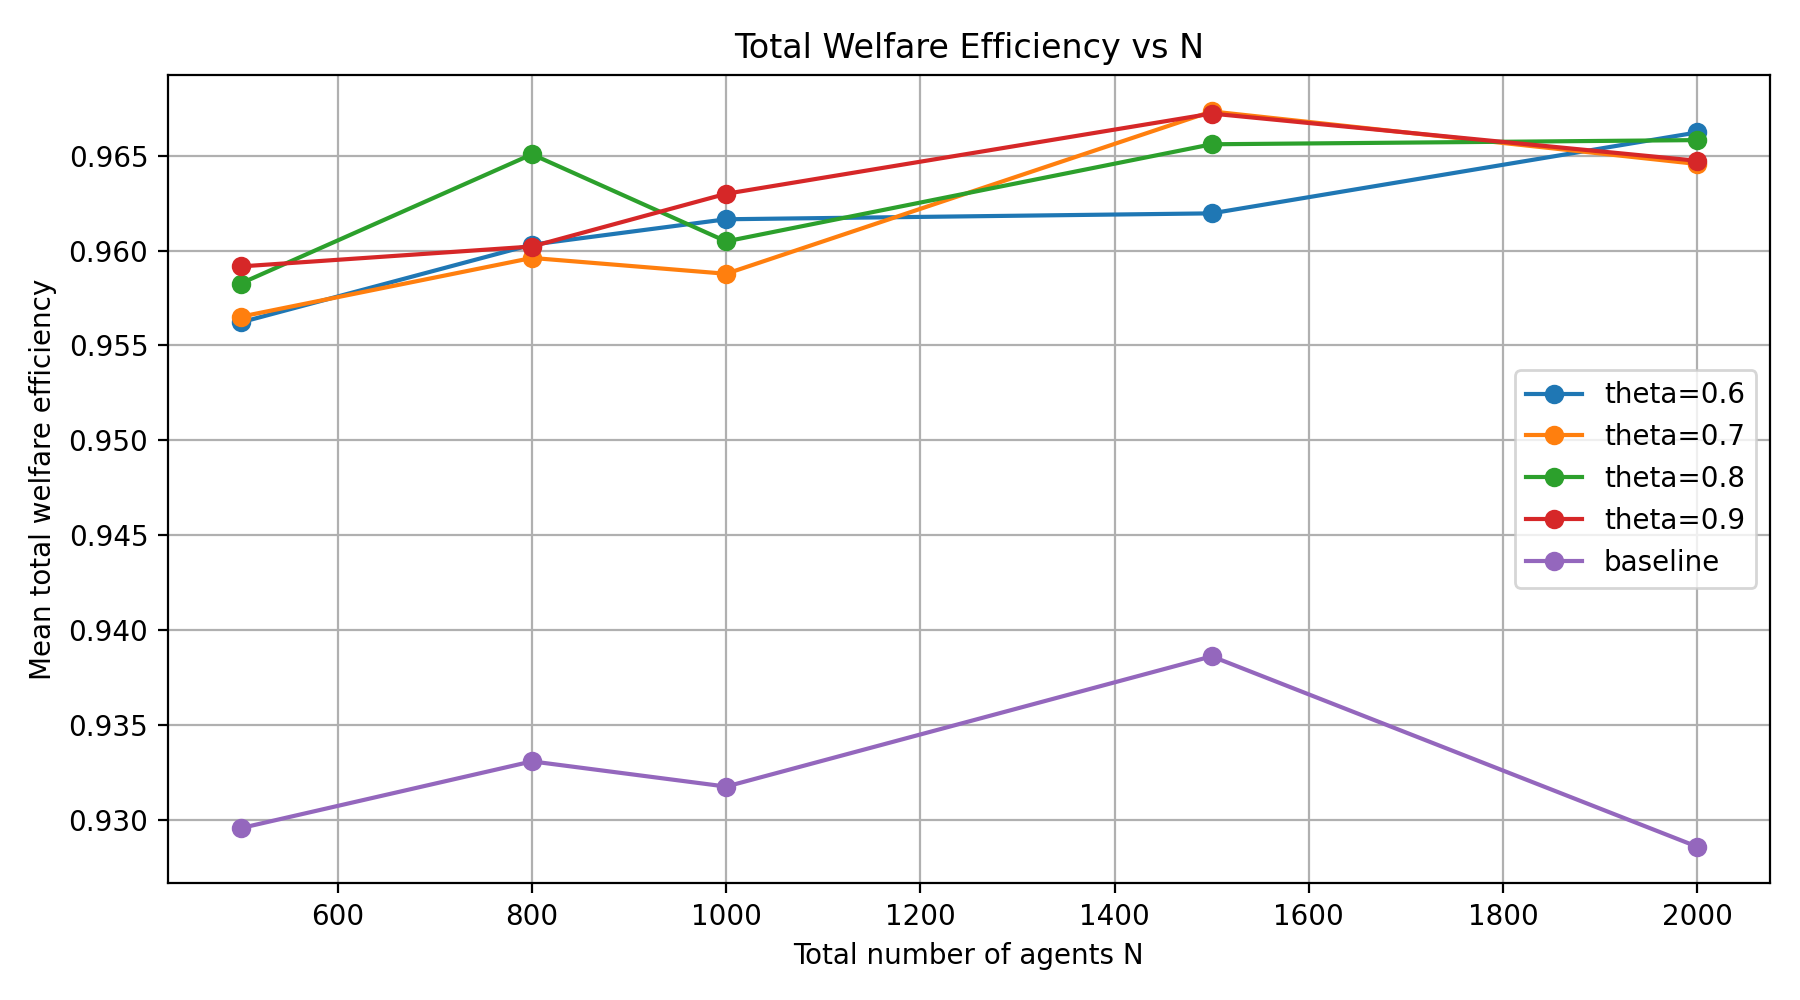
\includegraphics[width=0.82\textwidth]{mean_total_efficiency_vs_N.png}
    \caption{不同市场规模下的总社会福利效率}
    \label{fig:mean_total_efficiency}
\end{figure}

图 \ref{fig:mean_total_efficiency} 显示，启用 balance 后，总社会福利效率整体高于 baseline。但由于总福利包含卖方初始持有商品带来的基础福利，因此该指标只能作为辅助参考。

\begin{figure}[h]
    \centering
    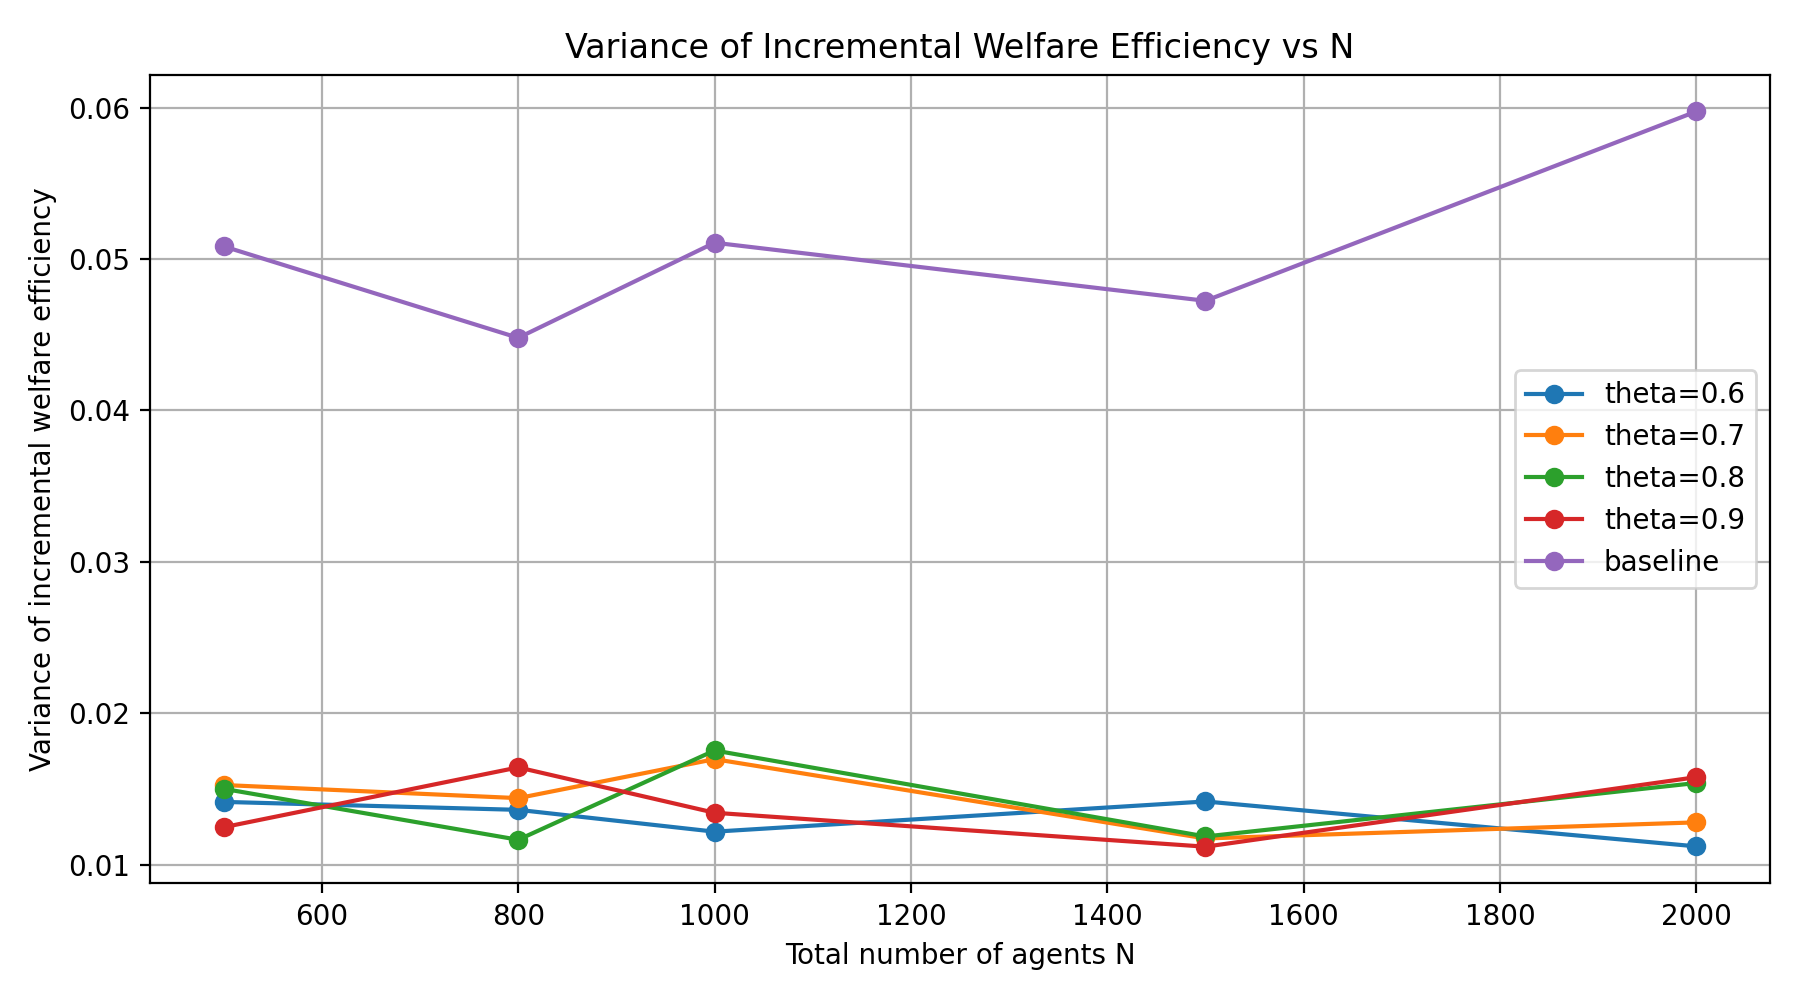
\includegraphics[width=0.82\textwidth]{var_surplus_efficiency_vs_N.png}
    \caption{不同市场规模下增量社会福利效率的方差}
    \label{fig:var_surplus_efficiency}
\end{figure}

图 \ref{fig:var_surplus_efficiency} 显示，baseline 的增量福利效率方差明显高于 balance 机制。这意味着在不进行动态补充时，机制表现更依赖随机网络结构；若某些层严重失衡，成交效率会显著下降。Balance 机制通过从下一层补充缺失方，降低了随机网络结构带来的波动，使平台表现更加稳定。

\subsection{实验结论}

仿真结果支持以下结论：

\begin{enumerate}
    \item 动态 balance 扩容能够提高平均成交数量；
    \item 动态 balance 扩容能够提高增量社会福利效率；
    \item 动态 balance 扩容能够降低机制对随机网络结构的敏感性；
    \item balance 阈值并非越高越好，实际部署中应根据市场成熟度、品类流动性和补充成本灵活设置。
\end{enumerate}

因此，balance 机制适合作为基础双边扩散拍卖的效率优化模块，而不是替代基础机制的独立机制。

\section*{结语}
\addcontentsline{toc}{section}{结语}

inFDT 的核心不是做一个普通信息撮合平台，而是构建一个面向稀缺数字资源与金融资源的可信交易基础设施。

平台通过信息传播扩大市场厚度，通过双边拍卖形成动态价格，通过标签化分类处理非完全同质资源，通过信用指数和 Sybil 风控降低小号操控与虚假交易风险。

在早期阶段，inFDT 应聚焦 AI 算力时间片、Agent 任务执行名额和应收账款与票据收益权三个主场景，先验证交易闭环和机制价值，再逐步拓展到 API 优先调用权、专家审核时间片、本地模型贡献名额、未来数据采集任务和 AI 安全红队测试等更多场景。

最终，inFDT 有机会从单一交易撮合工具发展为集交易撮合、价格发现、信用风控和智能分类于一体的金融科技基础设施。

\end{document}
